\section{Experimentation and Results}
\subsection{Datasets}
\textbf{arXiv corpus.} The 27~October~2026 arXiv metadata snapshot, filtered to
papers listed in cs.CL, cs.LG, cs.AI or cs.IR and first submitted between January
2023 and October 2026: \NDocs{} titles and abstracts and \NTerms{} index terms.
\textbf{Fresh-2026.} We requested 201 sampled papers before arXiv began throttling
the crawler. \NCrawled{} had an HTML version, and \NPapers{} produced at least one
valid query, giving \NFresh{} queries: \NDev{} for tuning (dev) and \NTest{} for
testing. \NTermQ{} test queries contain an emerging term.
\textbf{LitSearch}~\cite{ajith2024}: 597 queries (inline-citation and author-written,
specific and broad) over \NLitDocs{} ACL/ICLR papers. We use the published titles and
abstracts and report recall@5 for specific and recall@20 for broad questions, as the
paper does.
\textbf{Term labels.} 230 terms were labelled as genuine new technical
terms or not: the top 60 detected terms, a random sample of 70 other detected terms,
60 rejected high-growth candidates, and a reference list of 40 well-known
2024--2026 terms. The origin links of \OriginNamed{} named artefacts (methods,
models, benchmarks, tools) were also checked.

\textbf{Setup.} All parameters are tuned on the Fresh-2026 dev split and then fixed;
LitSearch is never used for tuning. Everything runs on one laptop (Apple M4 Pro,
48\,GB). Mean latency per query over \NDocs{} papers is \LatBm{}\,ms for BM25 and
\LatFrontier{}\,ms for Frontier, including query encoding on the GPU
(Fig.~\ref{fig:lat}).

\subsection{Main results on Fresh-2026}
Table~\ref{tab:fresh} lists all systems on the test split. Frontier is best on every
metric: nDCG@10 \FrontierNdcg{}, against \HybridNdcg{} for the tuned hybrid,
\TfidfNdcg{} for TF-IDF, \BmNdcg{} for BM25 and \BgeNdcg{} for bge-small. The
improvement over the hybrid is significant ($p_t=\SigP$; better on \SigWins{}
queries, worse on \SigLosses{}). Fusion is the largest step among the baselines: it
adds 4 points over BM25 and 9 over bge-small, because lexical and dense retrievers
fail on different queries. The small 2023 embedders are weaker than BM25 on their
own on this domain, as BEIR~\cite{thakur2021} also found out of domain.
Table~\ref{tab:sig} gives all paired tests.

\begin{table}[t]
\centering\small\setlength{\tabcolsep}{4pt}
\caption{Fresh-2026 test split (\NTest{} queries, time-aware). $+E$ marks
emerging-term expansion. Best in bold.}
\label{tab:fresh}
\resizebox{\linewidth}{!}{\begin{tabular}{lrrrrrr}
\toprule
System & R@5 & R@20 & R@100 & nDCG@10 & MRR & MAP \\
\midrule
TF-IDF & 41.4 & 53.2 & 62.3 & 42.1 & 42.6 & 39.5 \\
QL-Dirichlet & 40.5 & 50.5 & 59.5 & 39.2 & 39.2 & 36.4 \\
BM25 & 42.4 & 50.9 & 59.5 & 40.9 & 41.2 & 38.2 \\
BM25{+}PRF & 42.1 & 50.7 & 58.8 & 39.4 & 39.3 & 36.4 \\
BM25{+}E & 43.1 & 51.4 & 60.0 & 41.4 & 41.7 & 38.7 \\
e5-small & 34.3 & 44.9 & 53.0 & 31.1 & 31.3 & 28.4 \\
e5-small{+}E & 34.7 & 45.4 & 55.6 & 32.0 & 32.4 & 29.2 \\
bge-small & 39.1 & 48.4 & 58.6 & 36.3 & 36.9 & 33.0 \\
bge-small{+}E & 39.1 & 49.5 & 59.3 & 36.7 & 37.4 & 33.6 \\
Hybrid & 46.3 & 57.4 & 69.4 & 45.0 & 46.1 & 42.9 \\
Hybrid{+}E & 47.7 & 57.9 & 69.9 & 45.8 & 46.4 & 43.4 \\
Frontier & \textbf{49.5} & \textbf{60.0} & \textbf{70.8} & \textbf{47.8} & \textbf{48.5} & \textbf{45.1} \\
\bottomrule
\end{tabular}
}
\end{table}

\begin{figure}[t]
\centering
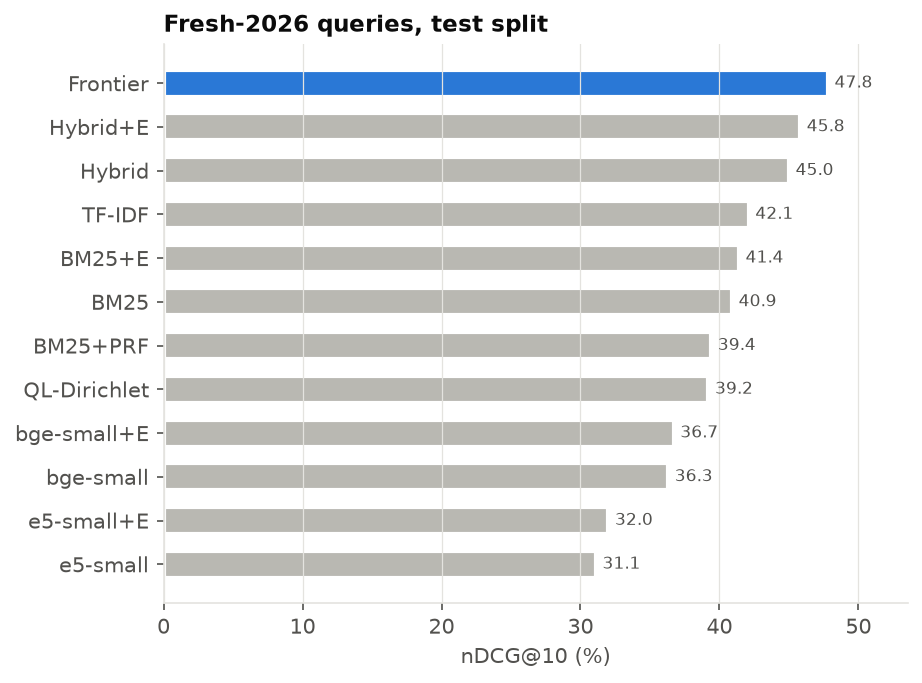
\includegraphics[width=\linewidth]{../results/figs/fresh_ndcg.png}
\caption{nDCG@10 on the Fresh-2026 test split.}
\label{fig:freshbar}
\end{figure}

\subsection{Effect of emerging terms}
Table~\ref{tab:hasterm} and Fig.~\ref{fig:hasterm} split the test queries by whether
they contain an emerging term.

\textbf{(1) All baselines struggle on new vocabulary.} BM25 drops from \NoTermBm{}
to \TermBm{} nDCG@10. Emerging terms are not rare tokens: GRPO appears in 1{,}800
papers and Qwen3 in hundreds, so they get a low IDF and match many papers that merely
\emph{use} the term. The cited paper, however, is usually the one that
\emph{introduced} it. The dense models also lose 10--18 points.

\textbf{(2) Expansion helps every retriever}: BM25 \TermBm{} $\rightarrow$
\TermBmE{}, bge-small \TermBge{} $\rightarrow$ \TermBgeE{}, e5-small \TermEfive{}
$\rightarrow$ \TermEfiveE{}, hybrid \TermHybrid{} $\rightarrow$ \TermHybridE{}. The
gains are consistent, but with \NTermQ{} queries none is significant on its own.

\textbf{(3) Origin linking gives the largest gain}: Frontier reaches \TermFrontier{}
on these queries, \textbf{+12.6 points over the hybrid} ($p_t=\TermSigP$, better on
\TermSigWins{} queries, worse on \TermSigLosses{}). Linking a named term to its
introducing paper is exactly what an inline citation needs.

\textbf{(4) No harm elsewhere}: on queries without emerging terms Frontier equals the
hybrid (\NoTermFrontier{} vs.\ \NoTermHybrid{}), because the layer only switches on
when a term is found.

\begin{table}[t]
\centering\small
\caption{nDCG@10 on test queries with and without an emerging term.}
\label{tab:hasterm}
\begin{tabular}{lrr}
\toprule
System & no emerging term & emerging term \\
\midrule
BM25 & 46.7 & 19.9 \\
bge-small & 38.4 & 28.6 \\
e5-small & 35.0 & 16.9 \\
Hybrid & \textbf{49.9} & 27.4 \\
Hybrid{+}E & \textbf{49.9} & 31.1 \\
Frontier & \textbf{49.9} & \textbf{40.0} \\
\bottomrule
\end{tabular}

\end{table}

\begin{figure}[t]
\centering
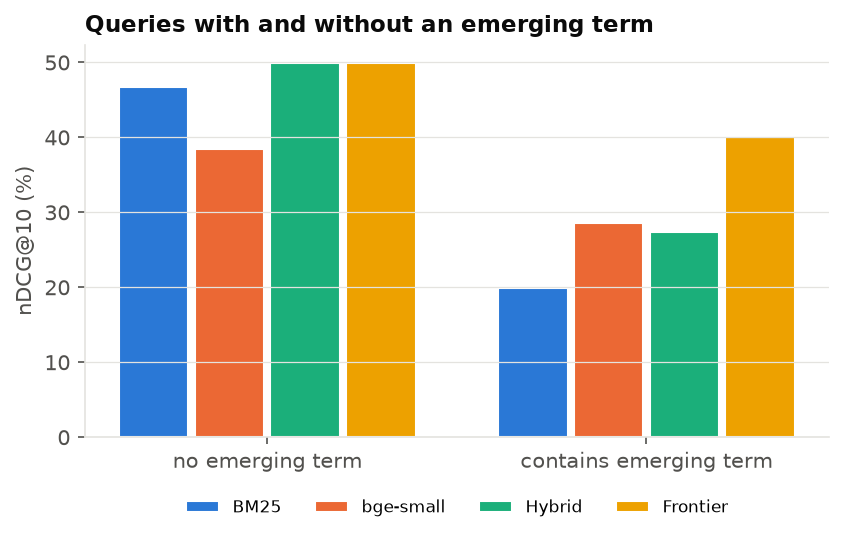
\includegraphics[width=\linewidth]{../results/figs/has_term.png}
\caption{nDCG@10 by query type: every baseline drops on new vocabulary; Frontier
recovers most of the gap.}
\label{fig:hasterm}
\end{figure}

\textbf{Age of the cited paper.} Table~\ref{tab:era} splits queries by when the cited
paper appeared. Every system finds queries about \emph{new} papers (after July 2025)
easier, because recent work is usually cited by a distinctive name. The gap between
BM25 and the 2023 dense model, however, is widest exactly there: \EraNewBm{} vs.\
\EraNewBge{} for new papers, against \EraOldBm{} vs.\ \EraOldBge{} for papers from
before July 2024. This fits the vocabulary drift that motivates our work. Frontier is
best in every age group.

\begin{table}[t]
\centering\small
\caption{nDCG@10 by publication date of the cited paper (test split).}
\label{tab:era}
\begin{tabular}{lrrr}
\toprule
System & before 2024-07 & mixed & after 2025-07 \\
\midrule
BM25 & 34.8 & 34.1 & 59.2 \\
bge-small & 29.8 & 32.7 & 50.4 \\
e5-small & 26.5 & 24.1 & 47.8 \\
Hybrid & 37.4 & 38.9 & 64.6 \\
Hybrid{+}E & 37.7 & 41.2 & 64.1 \\
Frontier & \textbf{40.4} & \textbf{42.7} & \textbf{65.4} \\
\bottomrule
\end{tabular}

\end{table}

\begin{table*}[t]
\centering\small
\caption{Paired significance tests on the Fresh-2026 test split. W/L = queries
where A is better / worse than B; $p_t$ paired t-test, $p_W$ Wilcoxon signed-rank.}
\label{tab:sig}
\begin{tabular}{llrrrrr}
\toprule
Comparison & Metric & Mean A & Mean B & W/L & $p_t$ & $p_W$ \\
\midrule
Frontier vs Hybrid & nDCG@10 & 47.8 & 45.0 & 14/3 & 0.013 & 0.010 \\
Frontier vs Hybrid & R@20 & 60.0 & 57.4 & 6/1 & 0.027 & 0.019 \\
Frontier vs BM25 & nDCG@10 & 47.8 & 40.9 & 43/19 & 2e-5 & 3e-5 \\
Frontier vs BM25 & R@20 & 60.0 & 50.9 & 24/3 & 2e-5 & 3e-5 \\
Frontier vs bge-small & nDCG@10 & 47.8 & 36.3 & 72/15 & 3e-8 & 3e-8 \\
Frontier vs bge-small & R@20 & 60.0 & 48.4 & 39/8 & 4e-6 & 1e-5 \\
Hybrid{+}E vs Hybrid & nDCG@10 & 45.9 & 45.0 & 9/3 & 0.177 & 0.147 \\
Hybrid{+}E vs Hybrid & R@20 & 57.9 & 57.4 & 2/2 & 0.528 & 0.458 \\
BM25{+}E vs BM25 & nDCG@10 & 41.4 & 40.9 & 5/1 & 0.144 & 0.075 \\
BM25{+}E vs BM25 & R@20 & 51.4 & 50.9 & 1/0 & 0.318 & 0.317 \\
bge-small{+}E vs bge-small & nDCG@10 & 36.7 & 36.3 & 8/7 & 0.616 & 0.570 \\
bge-small{+}E vs bge-small & R@20 & 49.5 & 48.4 & 5/3 & 0.298 & 0.248 \\
Hybrid vs BM25 & nDCG@10 & 45.0 & 40.9 & 35/19 & 0.001 & 0.002 \\
Hybrid vs BM25 & R@20 & 57.4 & 50.9 & 20/4 & 9e-4 & 0.001 \\
\bottomrule
\end{tabular}

\end{table*}

\subsection{Comparison with a published paper: LitSearch}
Table~\ref{tab:lit} compares our systems with the results published in
LitSearch~\cite{ajith2024}, using the same queries, corpus and metrics. Our BM25
(stemming, title zone, $k_1,b$ tuned on Fresh-2026) reaches \LitBm{} recall@5 on
specific questions, against 50.0 published. Our hybrid of BM25 and the 33M-parameter
bge-small reaches \LitHybrid{} (broad recall@20 \LitBroadHybrid{}). This beats the
published E5-large-v2 (56.2/55.4) and Instructor-XL (52.3/56.5), and narrows the gap
to GritLM-7B (74.8/70.8), a model about 200 times larger.
LitSearch's papers predate our emerging terms: only \LitTermQ{} of its 597 queries
contain one, and no origin links exist in that corpus. Frontier therefore behaves
exactly like the hybrid there (\LitFrontier{}), which shows the new layer is safe on
older literature. The PageRank prior leaves recall@5 unchanged but gives a small,
significant nDCG@10 gain (\LitFrontierNdcg{} $\rightarrow$ \LitPrNdcg{},
$p_t=\LitPrP$). Citation authority helps break ties between candidates.

\begin{table*}[t]
\centering\small
\caption{LitSearch: our systems (top) against the published results of
Ajith et al.~\cite{ajith2024} (bottom). Recall@5 for specific and recall@20 for broad
questions, titles and abstracts only.}
\label{tab:lit}
\begin{tabular}{lrrrrrr}
\toprule
System & \multicolumn{2}{c}{Inline-citation} & \multicolumn{2}{c}{Author-written} & \multicolumn{2}{c}{Average} \\
 & Spec.\ R@5 & Broad R@20 & Spec.\ R@5 & Broad R@20 & Spec.\ R@5 & Broad R@20 \\
\midrule
TF-IDF & 43.5 & 43.3 & 60.2 & 51.4 & 51.5 & 45.1 \\
QL-Dirichlet & 43.7 & 41.4 & 61.1 & 60.0 & 52.0 & 45.6 \\
BM25 & 46.5 & 44.6 & 65.9 & 57.1 & 55.8 & 47.5 \\
BM25{+}PRF & 41.8 & 45.9 & 63.0 & 57.1 & 51.9 & 48.4 \\
e5-small & 43.7 & 38.9 & 53.1 & 54.3 & 48.2 & 42.4 \\
bge-small & 51.9 & 59.4 & 55.5 & 57.1 & 53.6 & 58.9 \\
Hybrid & 55.6 & 58.3 & 73.5 & 68.6 & 64.1 & 60.6 \\
Frontier & 55.6 & 58.3 & 73.5 & 68.6 & 64.1 & 60.6 \\
Frontier{+}PageRank & 56.5 & 58.3 & 72.5 & 65.7 & 64.1 & 60.0 \\
\midrule
BM25 \cite{ajith2024} & 38.5 & 37.4 & 62.6 & 48.6 & 50.0 & 39.9 \\
GTR-T5-large \cite{ajith2024} & 38.5 & 45.7 & 40.8 & 37.1 & 39.6 & 43.8 \\
Instructor-XL \cite{ajith2024} & 48.9 & 56.3 & 55.9 & 57.1 & 52.3 & 56.5 \\
E5-large-v2 \cite{ajith2024} & 50.4 & 55.8 & 62.6 & 54.3 & 56.2 & 55.4 \\
GritLM-7B \cite{ajith2024} & 67.7 & 69.7 & 82.5 & 74.3 & 74.8 & 70.8 \\
\bottomrule
\end{tabular}

\end{table*}

\begin{figure}[t]
\centering
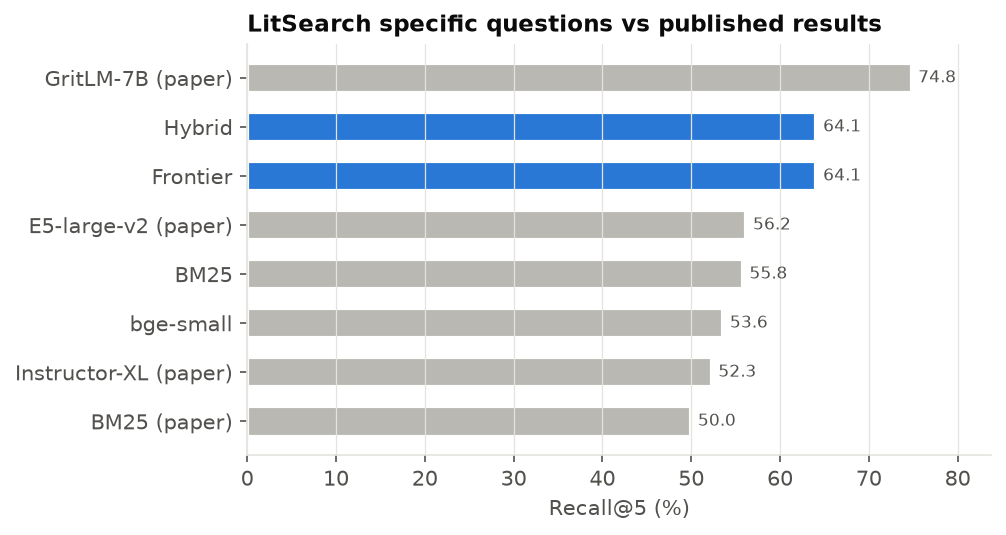
\includegraphics[width=\linewidth]{../results/figs/litsearch.png}
\caption{LitSearch specific questions: ours (blue) vs.\ published retrievers.}
\label{fig:lit}
\end{figure}

\subsection{Emerging-term detection and linking}
Table~\ref{tab:terms} scores term detection as a classification against the labels.
Precision is high among the top-ranked terms (\TopP{}) and lower in the long tail
(\RandP{} on a random sample of the rest). The detector recovers \RefR{} of the
reference terms and correctly rejects \RejAcc{} of the high-growth generic
candidates. The missed reference terms are mostly older ones whose burst began before
July 2024, such as \emph{test-time scaling} and \emph{LLM-as-a-judge}.
Origin linking is correct for \OriginCorrect{} of the \OriginNamed{} named
artefacts, i.e.\ \OriginAccOn{}\% of those whose introducing paper is on arXiv.
Examples: GRPO $\rightarrow$ DeepSeekMath, Qwen3-4B $\rightarrow$ Qwen3 Technical
Report, DAPO, GSPO, GEPA, DeepSeek-R1/V3, SWE-bench, BrowseComp, HarmBench, SGLang
and FineWeb-Edu. Product names announced outside arXiv (GPT-5.x, Claude Code, MCP)
are linked to an early paper about them instead. Context-based disambiguation is
essential here. Without it, MCP was linked to a 2023 \emph{Mass-Conserving
Perceptron}, DAPO to an unrelated \emph{Dual Approximation Policy Optimization}, and
LLaDA to a driving paper. Fig.~\ref{fig:bursts} shows detected bursts.

\begin{table}[t]
\centering\small\setlength{\tabcolsep}{4pt}
\caption{Emerging-term detection against manual labels.}
\label{tab:terms}
\begin{tabular}{lrrrrr}
\toprule
Set & $n$ & P & R & F1 & Acc. \\
\midrule
Top-60 detected & 60 & 0.61 & -- & -- & -- \\
Random detected & 70 & 0.22 & -- & -- & -- \\
Reference list & 40 & -- & 0.65 & -- & -- \\
Rejected & 60 & -- & -- & -- & 0.98 \\
Combined & 169 & 0.43 & 0.71 & 0.54 & 0.59 \\
\bottomrule
\end{tabular}

\end{table}

\begin{figure}[t]
\centering
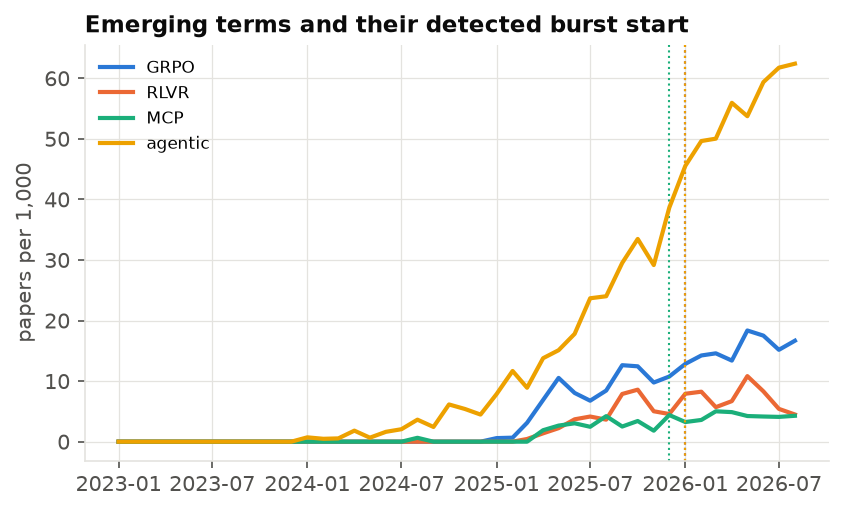
\includegraphics[width=\linewidth]{../results/figs/bursts.png}
\caption{Monthly rate of four emerging terms; dotted lines mark the start of the
latest burst found by Kleinberg's automaton.}
\label{fig:bursts}
\end{figure}

\begin{figure}[t]
\centering
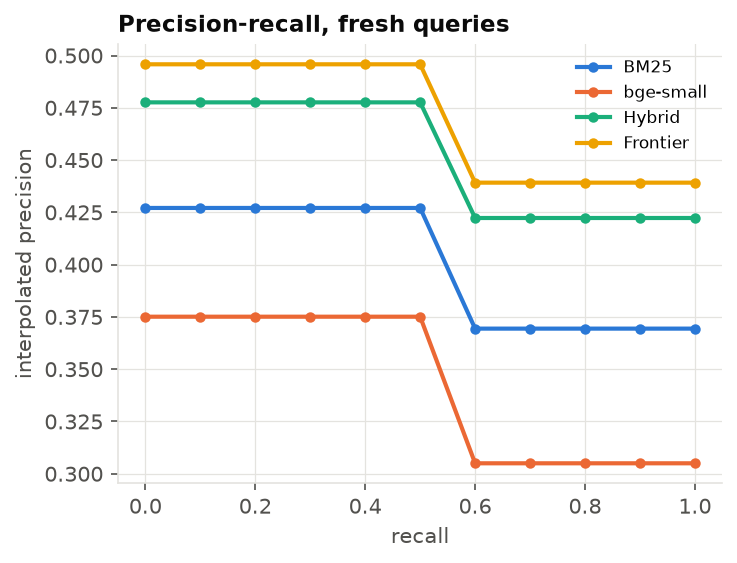
\includegraphics[width=0.49\linewidth]{../results/figs/pr_fresh.png}
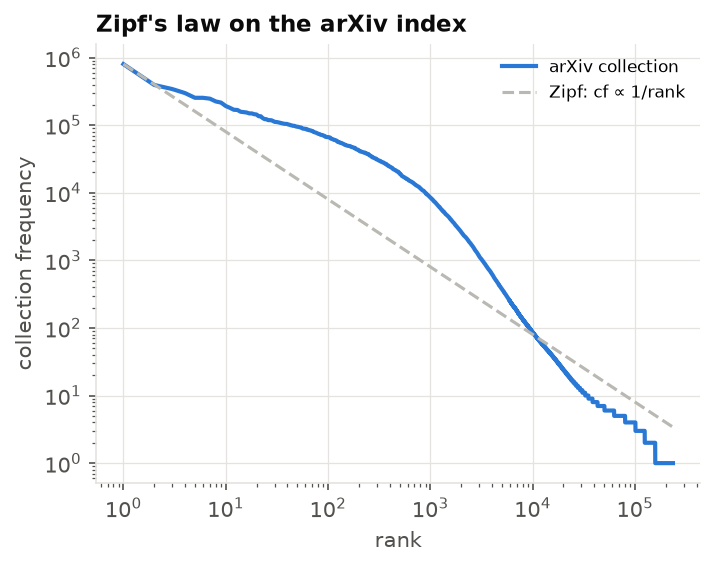
\includegraphics[width=0.49\linewidth]{../results/figs/zipf.png}
\caption{Left: interpolated precision--recall on Fresh-2026. Right: Zipf's law on
the arXiv index.}
\label{fig:zipf}
\end{figure}

\begin{figure}[t]
\centering
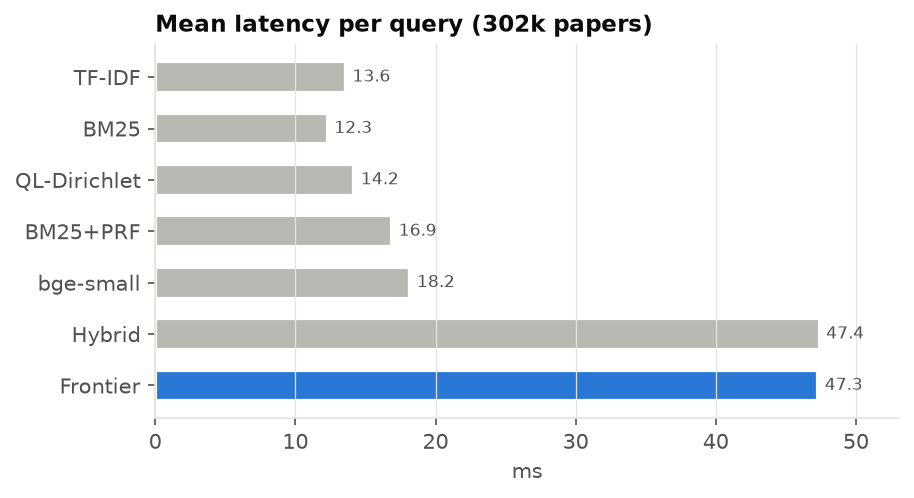
\includegraphics[width=0.9\linewidth]{../results/figs/latency.png}
\caption{Mean latency per query over \NDocs{} papers.}
\label{fig:lat}
\end{figure}

\subsection{Discussion}
Three lessons stand out. First, classic IR does most of the work. A tuned BM25 is a
strong baseline, and a simple min-max fusion with a small embedder beats much larger
dense models on LitSearch. Second, new vocabulary is a real weakness of \emph{both}
retriever families, but for different reasons. Lexical matching cannot tell which of
the many papers using a popular new term is meant. Dense models trained before the
term existed do not know what it means. Third, the most effective fix is not
richer matching but \emph{knowledge}: knowing which paper introduced a term. Tuning
on the dev split chose a strong origin boost ($\lambda=\CfgLink$) with light
expansion ($\beta=\CfgBeta$). It kept the same fusion weight with or without an
emerging term ($\alpha_E=\alpha=\CfgAlpha$), so the adaptive-fusion component turned
out to be unnecessary once expansion and linking were in place. The gains cost
nothing at query time: Frontier's latency equals the hybrid's (\LatHybrid{}\,ms).

\section{Conclusions and Limitations}
We built Frontier, a complete search engine for the latest AI research. Detecting
emerging terms from corpus statistics, and linking them to the papers that
introduced them, improves retrieval significantly. It adds +12.6 nDCG@10 on queries
with new vocabulary and +2.8 overall over a tuned hybrid, without retraining any
model or calling an LLM at query time. Our hybrid baseline also beats several much
larger published retrievers on LitSearch.

\textbf{Limitations.}
(1) Fresh-2026 is built automatically: a citation sentence is an imperfect query, an
author may cite one of several valid papers, and unresolved citations are dropped.
With \NTest{} test queries (\NTermQ{} with emerging terms), small differences are not
significant.
(2) The title-prefix and model-family rules for origin linking were added after
inspecting linking errors on Fresh-2026 queries from both splits. The test-split
gain of the origin boost may therefore be slightly optimistic.
(3) Term detection is noisy in the long tail (precision \RandP{}). The labels
come from the project itself, not from independent annotators.
(4) Origins cannot be found for terms introduced outside arXiv (blogs, product
launches).
(5) We use small 2023 embedders because of laptop compute. Newer models (e.g.\
Qwen3-Embedding) would raise all dense numbers, but their own training cutoff moves
the vocabulary gap rather than closing it.
(6) We index titles and abstracts only. arXiv HTML crawling at the required 15\,s
delay, plus throttling, limited Fresh-2026 to \NPapers{} citing papers.
\textbf{Future work}: extracting definitions for glossary entries without an LLM,
term-aware document expansion at index time, and a continuously refreshed benchmark.
